\documentclass[10pt,border=1pt]{standalone}
\usepackage[T1]{fontenc}
\usepackage{mathpazo}
\usepackage{amsmath,amssymb}
\usepackage{xcolor}
\usepackage{pgfplots}
\pgfplotsset{compat=1.18}
\usetikzlibrary{shapes.geometric,positioning,arrows.meta,calc}
\definecolor{okorange}{HTML}{E69F00}
\definecolor{oksky}{HTML}{56B4E9}
\definecolor{okgreen}{HTML}{009E73}
\definecolor{okblue}{HTML}{0072B2}
\definecolor{okverm}{HTML}{D55E00}
\definecolor{okpurple}{HTML}{CC79A7}
\colorlet{accent}{okverm}
\pgfplotsset{
  safenest/.style={
    tick label style={font=\footnotesize},
    label style={font=\small},
    title style={font=\small, align=left},
    legend style={font=\footnotesize, draw=none, fill=none, cells={anchor=west}},
    grid style={black!12, line width=0.3pt},
    axis line style={black!70, line width=0.4pt},
    tick style={black!70, line width=0.4pt},
    axis lines*=left,
  },
}
\newlength{\figwidth}
\tikzset{every node/.append style={execute at begin node={\hyphenpenalty=10000\exhyphenpenalty=10000\relax}}}
\setlength{\figwidth}{18.47cm}
\begin{document}
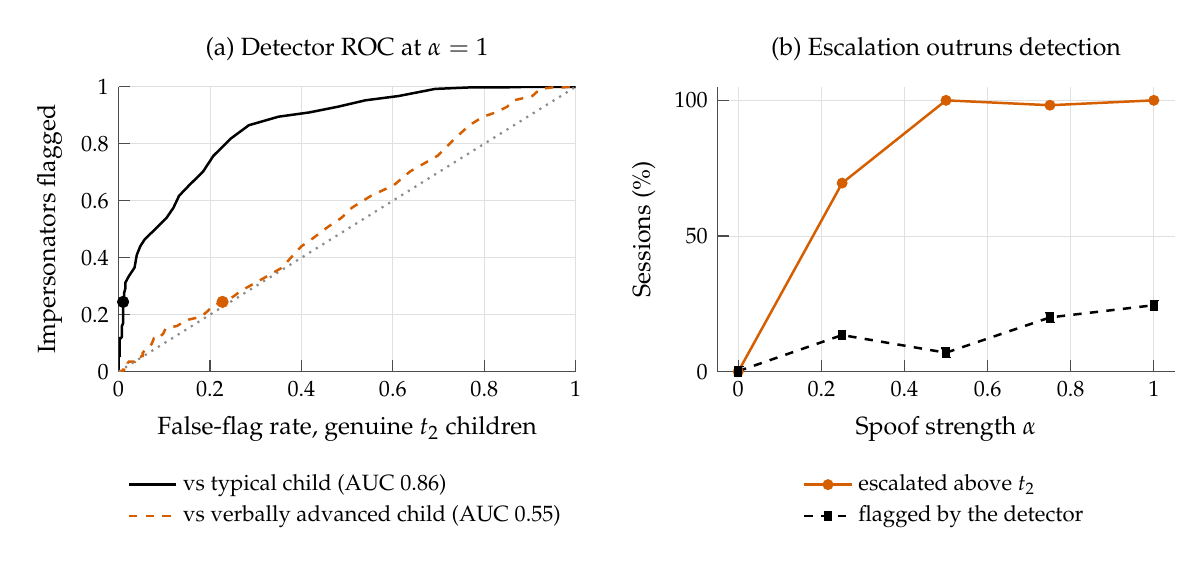
\begin{tikzpicture}
\begin{axis}[safenest, name=l, width=0.40\figwidth, height=52mm,
  xmin=0, xmax=1, ymin=0, ymax=1,
  xlabel={False-flag rate, genuine $t_2$ children}, ylabel={Impersonators flagged},
  xmajorgrids, ymajorgrids, title={(a) Detector ROC at $\alpha=1$},
  legend style={at={(0.5,-0.32)}, anchor=north, legend columns=1},
]
\addplot[black, line width=0.9pt] coordinates {(0.0000,0.0000) (0.0000,0.0025) (0.0000,0.0050) (0.0000,0.0075) (0.0000,0.0125) (0.0000,0.0150) (0.0000,0.0175) (0.0000,0.0200) (0.0000,0.0225) (0.0000,0.0250) (0.0000,0.0275) (0.0000,0.0300) (0.0000,0.0350) (0.0000,0.0400) (0.0000,0.0500) (0.0000,0.0525) (0.0025,0.0550) (0.0025,0.0625) (0.0025,0.0650) (0.0025,0.0700) (0.0025,0.0850) (0.0025,0.0975) (0.0025,0.1175) (0.0050,0.1175) (0.0075,0.1225) (0.0075,0.1325) (0.0075,0.1500) (0.0075,0.1575) (0.0075,0.1600) (0.0100,0.1700) (0.0100,0.1825) (0.0100,0.1925) (0.0100,0.2125) (0.0100,0.2300) (0.0100,0.2450) (0.0125,0.2475) (0.0125,0.2625) (0.0125,0.2775) (0.0150,0.2925) (0.0150,0.3125) (0.0225,0.3350) (0.0350,0.3650) (0.0400,0.4100) (0.0475,0.4400) (0.0575,0.4650) (0.0850,0.5075) (0.1050,0.5400) (0.1200,0.5750) (0.1325,0.6175) (0.1550,0.6550) (0.1850,0.7025) (0.2075,0.7575) (0.2450,0.8175) (0.2850,0.8650) (0.3500,0.8950) (0.4175,0.9100) (0.4800,0.9300) (0.5400,0.9525) (0.6125,0.9675) (0.6925,0.9925) (0.7650,0.9975) (0.8325,0.9975) (0.9025,1.0000) (0.9650,1.0000) (0.9925,1.0000) (1.0000,1.0000)};
\addlegendentry{vs typical child (AUC 0.86)}
\addplot[accent, dashed, line width=0.9pt] coordinates {(0.0000,0.0000) (0.0050,0.0025) (0.0075,0.0025) (0.0100,0.0025) (0.0100,0.0050) (0.0100,0.0075) (0.0125,0.0075) (0.0125,0.0125) (0.0125,0.0150) (0.0150,0.0150) (0.0150,0.0175) (0.0175,0.0175) (0.0175,0.0200) (0.0175,0.0225) (0.0175,0.0250) (0.0200,0.0250) (0.0200,0.0275) (0.0200,0.0300) (0.0225,0.0350) (0.0250,0.0350) (0.0275,0.0350) (0.0300,0.0350) (0.0350,0.0350) (0.0350,0.0400) (0.0400,0.0500) (0.0450,0.0525) (0.0475,0.0525) (0.0525,0.0550) (0.0525,0.0625) (0.0525,0.0650) (0.0550,0.0700) (0.0650,0.0850) (0.0725,0.0975) (0.0775,0.1175) (0.0825,0.1175) (0.0825,0.1225) (0.0900,0.1225) (0.0975,0.1325) (0.1025,0.1500) (0.1175,0.1575) (0.1275,0.1600) (0.1375,0.1700) (0.1525,0.1825) (0.1800,0.1925) (0.1950,0.2125) (0.2050,0.2300) (0.2275,0.2450) (0.2325,0.2475) (0.2500,0.2625) (0.2625,0.2775) (0.2775,0.2925) (0.3000,0.3125) (0.3250,0.3350) (0.3575,0.3650) (0.3825,0.4100) (0.4000,0.4400) (0.4225,0.4650) (0.4575,0.5075) (0.4875,0.5400) (0.5100,0.5750) (0.5525,0.6175) (0.6025,0.6550) (0.6375,0.7025) (0.6975,0.7575) (0.7350,0.8175) (0.7675,0.8650) (0.7975,0.8950) (0.8250,0.9100) (0.8500,0.9300) (0.8650,0.9525) (0.9050,0.9675) (0.9225,0.9925) (0.9475,0.9975) (0.9700,0.9975) (0.9875,1.0000) (1.0000,1.0000) (1.0000,1.0000)};
\addlegendentry{vs verbally advanced child (AUC 0.55)}
\addplot[black!45, dotted, line width=0.8pt, forget plot] coordinates {(0,0) (1,1)};
\addplot[only marks, mark=*, mark size=2pt, black, forget plot] coordinates {(0.0100,0.2450)};
\addplot[only marks, mark=*, mark size=2pt, accent, forget plot] coordinates {(0.2275,0.2450)};
\end{axis}
\begin{axis}[safenest, at={($(l.east)+(18mm,0)$)}, anchor=west,
  width=0.40\figwidth, height=52mm,
  xmin=-0.05, xmax=1.05, ymin=0, ymax=105,
  xlabel={Spoof strength $\alpha$}, ylabel={Sessions (\%)},
  xmajorgrids, ymajorgrids, title={(b) Escalation outruns detection},
  legend style={at={(0.5,-0.32)}, anchor=north, legend columns=1},
]
\addplot[mark=*, mark size=1.5pt, accent, line width=0.9pt] coordinates {(0.0,0.0) (0.25,69.5) (0.5,100.0) (0.75,98.2) (1.0,100.0)};
\addlegendentry{escalated above $t_2$}
\addplot[mark=square*, mark size=1.5pt, black, dashed, line width=0.9pt] coordinates {(0.0,0.2) (0.25,13.5) (0.5,7.0) (0.75,20.0) (1.0,24.5)};
\addlegendentry{flagged by the detector}
\end{axis}
\end{tikzpicture}
\end{document}
